\documentclass{article}


\usepackage{arxiv}

\usepackage[utf8]{inputenc} % allow utf-8 input
\usepackage[T1]{fontenc}    % use 8-bit T1 fonts
\usepackage{hyperref}       % hyperlinks
\usepackage{url}            % simple URL typesetting
\usepackage{booktabs}       % professional-quality tables
\usepackage{amsfonts}       % blackboard math symbols
\usepackage{nicefrac}       % compact symbols for 1/2, etc.
\usepackage{microtype}      % microtypography
\usepackage{tabularx}
\usepackage{lipsum}

\usepackage{mathtools}
\DeclarePairedDelimiter\ceil{\lceil}{\rceil}
\DeclarePairedDelimiter\floor{\lfloor}{\rfloor}
\DeclareMathOperator*{\argmax}{arg\,max}
\DeclareMathOperator*{\argmin}{arg\,min}




\usepackage{cite}
\let\proof\relax
\let\endproof\relax
\usepackage{amsmath,amssymb,amsthm}


\newtheorem{theorem}{Theorem}
\newtheorem{lemma}{Lemma}
\newtheorem{corollary}{Corollary}
\newtheorem*{remark*}{Remark}
\newtheorem{assumption}{Assumption}
\newtheorem{definition}{Definition}
\newtheorem{conjecture}{Conjecture}
\newtheorem*{conjecture*}{Conjecture}
\newtheorem{prop}{Proposition}
\newtheorem{example}{Example}
\newtheorem*{problem*}{Problem}
\usepackage[linesnumbered]{algorithm2e}
\usepackage{graphicx}
\usepackage{textcomp}



\title{K-foggy Sequences}


\author{
  Elad Michael   
   \And
  Johan Lennart Westin \\
  \And
  Austin Polanco \\
  \And
  /u/supermac30 \\ % TODO - Add your real name if you dare
}

\begin{document}
\maketitle

\begin{abstract}
	% TODO: Move all links to intro, and be more specific here on what we study (periods, etc.)
	Exploring the properties of $k$-foggy sequences, as described by /u/supermac30 in their \href{https://www.reddit.com/r/math/comments/gdsjth/foggy_sequences/}{Reddit post}. See also \href{https://oeis.org/A334539}{OEIS entry A334539}.
\end{abstract}

% keywords can be removed
%\keywords{Number Theory \and Look and Say \and Foggy Sequence}


% \section*{JWson's Suggestion Corner}

% Here are some proposals for notation changes, let me know if you agree.

% \begin{itemize}
% 	\item Change the counting function $\mathcal{C}$ to $\mathcal{N}$ or $\mathcal{C}$, which would look more intuitive in my opinion.
% 	\item Denote sequence terms with $a_k(i)$ rather than $a_i$.
% 	\item Denote sequence ranges with e.g. $a_k[i:j]$ rather than $a_{i:j}$.
% 	\item Use lower-case $k$ rather than $K$ for the $k$-foggy sequence identifier.
% 	\item Use lower-case "f" in "$k$-foggy" rather than "$k$-Foggy" or "$K$-Foggy."
% \end{itemize}


\section{A Foggy Introduction}
\label{sec:introduction}

Inspired by the Look and Say numbers, and the genius analysis by John Conway~\cite{thomas1987open}, the authors propose a sequence generator by the name of \emph{$k$-foggy}, for a given $k\in\mathbb{N}$. The sequences $a_{k}(n)$ is generated by the following rules:

% TODO - Express this definition as a conditional equation a_k(n) = { ...
\begin{enumerate}
	\item $a_k(n) := -1$ for all $n < 1$,
	\item $a_k(1) := 1$,
	\item Each subsequent term be $a_k(i+1) := \mathcal{C}_{a_k(i)}(a_k(i-k+1:i))$ where $\mathcal{C}_{m}(x)$ is a counting function that gives the number of times $m$ occurs in the sequence $x$.
\end{enumerate}

Casually described, the $i+1$-th term of the $k$-foggy sequence is the number of times the $i$-th term appears in the $k$ preceding terms. For example, in~\eqref{eq:5-foggyExample} we construct the $5$-foggy sequence to 30 terms.

\begin{equation}
	a_5 : 1,1,2,1,3,1,3,2,1,2,2,3,1,2,3,2,2,3,2,3,2,3,3,3,4,1,1,2,1,3,\dots \label{eq:5-foggyExample}
\end{equation}

We may immediately observe some interesting patterns in~\eqref{eq:5-foggyExample}, however we will not yet succumb to this temptation. The elements in the sequence~\eqref{eq:5-foggyExample} are all single digits, however they will not be in general, so we note that an element $a_i=17$ does not contribute to the counting of $1$ nor $7$, only to $17$. We may equivalently define each sequence in base $k$ to ensure single digits. If there are fewer than $k$ elements in the sequence, the counting ends at index $1$, or we may begin each sequence with a padding of $k-1$ zeros. We further borrow (steal) directly from Conway and define repetitions

% Is this notation necessary (i.e. will it be used)? 
% I was hoping to set conventions before we need them, to standardize our proofs. I have used the exponential notation a ton already in my proof attempts.
\begin{align*}
a^lb^m(cde)^n = \overbrace{a,...,a,}^{l}\overbrace{b,...,b,}^{m}\overbrace{c,d,e,c,d,e,...,c,d,e}^{3n}.
\end{align*} 

If we are excerpting from a sequence, we will use
\begin{itemize}
  \item $X$ - an arbitrary element,
  \item $X^{\neq n}$ - an arbitrary element not equal to $n$,
  \item $X^m$ - a sequence of $m$, not necessarily equal, arbitrary elements.
\end{itemize}

Where these many conventions are nested, or further complicated, the authors will endeavor to explain their meaning in the plainest terms.

% Maybe call this seciton something else ("basic properties" or something)?
\section{Warm-Ups}
\label{sec:warm-ups}

We begin with a few warm-up theorems, which serve to whet the appetite. 

\begin{definition}\label{def:ultimatelyPeriodic}
A sequence $S = s_1,s_2,s_3,s_4,...$ is ultimately periodic if there exists an index $t_0$ and a period $T$ such that $s_{t_0+k} = s_{t_0+k+T} \; \forall \; k \geq 0$. Note that are infinitely many valid periods $T$ (all integer multiples), we will always refer to the \emph{least} valid period $T$ as the period.
\end{definition}

% TODO - Suggestion of theorem order: 1) Prove all foggies are periodic, 2) prove the tight upper bound, 3) show period >= bound^k


\begin{theorem}\label{thm:allSequencesRepeat}
All $k$-foggy sequences are ultimately periodic with period no greater than $k^k$. 
\end{theorem}

\begin{proof}
The $i$-th term of the $k$-foggy sequence, for $i>k$, depends only on the $k$ preceding terms. By the pigeonhole principle, we have that the section $a_k(k^k : k^k+k)$ must exist elsewhere in the sequence. Let $t$ be the last index before $k^k$ such that $a_k(t:t+k) = a_k(k^k:k^k+k)$, then we have $a_k(t+k+1) = a_k(k^k+k+1)$ and in general $a_k(t+k+s) = a_k(k^k+k+s) \; \forall \; s \geq 0$. Therefore the sequence is periodic, with period $T_k= k^k - t \leq k^k$.
\end{proof}

Of course $k^k$ is an extremely conservative bound, for example the $5$-foggy sequence~\eqref{eq:5-foggyExample} has period $T_5 = 25 << 3125 = 5^5$.

\begin{lemma}\label{lem:longestRun}
Let $A$ be the longest consecutive run of an element $a_k(i)$ with a $k$-foggy sequence. Then the length of the run is bounded, i.e. $|A| \leq a_k(i) + 1$.
\end{lemma}

\begin{proof}
Assume there is an index $t$ such that $a_k(t)$ repeats $a_k(t) + 1$ times, i.e. $a_k(t:t+a_k(t)) = (a_k(t))^{a_k(t)+1}$. Then for the following term, by the definition of the $k$-foggy sequence, we have $a_k(t+a_k(t)+1)=\mathcal{C}_{a_k(t+a_k(t))}(a_k(t+a_k(t)-k+1:t+a_k(t))) \geq a_k(t)+1$, which is to say all $a_k(t) + 1$ are counted (assuming $a_k(t) \leq k$, which is trivially true), and thus the next term must be equal to or larger than $a_k(t) + 1$.  Therefore, we cannot have a repeated element $a_k(t)$ more than $a_k(t)+1$ times.
\end{proof}

\begin{lemma}\label{lem:twiceInARow}
No element $a_k(t) \geq \ceil{\frac{k}{2}}+1$ may appear twice in a row.
\end{lemma}

\begin{proof}
From the pigeonhole principle, if we have a sub-sequence $X^{\neq s},s,s$ where $s>\ceil{\frac{k}{2}}$, then the previous $k$ terms (before $X^{\neq s}$) must have contained $s$ occurences of $X^{\neq s}$. Therefore, including the first occurence of $s$, we have $s-1$ occurances of $X^{\neq s}$ and $s$ occurences of $s$, which gives $s-1+s \geq \ceil{\frac{k}{2}}+\ceil{\frac{k}{2}}+1 > k$, which is a contradiction.
\end{proof}

Note that Lemma~\ref{lem:twiceInARow} includes runs of longer than two, a fortiriori. 

\begin{theorem}\label{thm:elementUpperBound}
All elements of a $k$-foggy sequence have an upper bound of $\ceil{\frac{k}{2}}+1$.
\end{theorem}

\begin{proof}
Let $S_k = a_k(t-k+1:t)$ be the subsequence of length $k$ preceeding $a_k(t)$. We know that $S_k$ must contain $a_k(t) > \ceil{\frac{k}{2}}+1$ copies of $a_k(t-1)$. Let $a^*=a_k(t-1)$ be the repeated element. From Lemma~\ref{lem:twiceInARow}, we know that $a^*\leq \ceil{\frac{k}{2}}$, as otherwise it could appear only at every other position in $S_k$, which only $\ceil{frac{k}{2}}$ occurences. From Lemma~\ref{lem:longestRun}, we know that there cannot be more than $a^*+1$ occurences of $a^*$ in a row within $S_k$. After the initial set of $a^*+1$ occurences in $S_k$, all occurences of $a^*$ must be singletons, as the subsequent element is the count of occurences of $a^*$ which will be greater than $a^*+1$. Therefore, if $a_k(t)> \ceil{\frac{k}{2}}+2$, then there must be an $a^*$ in $S_k$ followed by $\ceil{\frac{k}{2}}+2$. It suffices then to prove that it is impossible to construct a sequence yeilding $a_k(t) = \ceil{\frac{k}{2}}+2$.

We begin by assuming the maximal value $a^* = \frac{k}{2}$. We first partition the subseqeunce $S_k$ as shown in~\eqref{eq:partitions1},
\begin{align}
S_k = [\overbrace{s_1,s_2,...,s_{l_1}}^{\mathcal{C}_{a^*}(S_k(1:l_1)) = a^*+1},X^{\neq a^*},a^*].\label{eq:partitions1}
\end{align}
In~\eqref{eq:partitions1}, we have partitioned the first $a^*+1$ occurences of s into the first $l_1$ elements, followed by an element not equal to $a^*$, followed by an $a^*$. In order for the $X^{\neq a^*}$ to be followed by an $a^*$, there must be $a^*$ occurences in the previous $k$ elements, along with the $a^*+1$ occurences of $a^*$ itself in the first $l_1$ elements. Therefore, we have that
\begin{align}
a^* + (a^*+1) &\leq k \\
a^* &\leq \frac{k}{2}-\frac{1}{2} 
\end{align}
which contradicts the assumption $a^*=\frac{k}{2}$. 

We generalize now by assuming s has value $a^* = \frac{k}{2}-i$. We then partition the subseqeunce $S_k$ as shown in~\eqref{eq:partitions2},
\begin{align}
S_k = [\overbrace{s_1,s_2,...,s_{l_1}}^{\mathcal{C}_{a^*}(S_k(1:l_1)) = a^*+1},(X^{\neq a^*},a^*)^{i},X^{\neq a^*},a^*].\label{eq:partitions2}
\end{align}
In order for the final $X^{\neq a^*}$ to be followed by an $a^*$, there must be $a^*$ occurences of it in the previous $k$ elements. Note that after every occurence of $a^*$, after the initial $l_1$ partition, the $X^{\neq a^*}$ is the running total of occurences of $a^*$ in $S_k$. Therefore, the terms $X^{\neq a^*}$ are unique, and summing the number of elements required to generate the final occurence of $a^*$ gives
\begin{align}
a^*+1+2i+a^* &\leq k\\
a^* \leq \frac{k}{2} - i - \frac{1}{2}
\end{align}
which contradicts the assumption that $a^* = \frac{k}{2}-i$.\\

This proof holds if the terms $X^{\neq a^*}$ are substituted for partitions of length $l_i$, containing any number of elements not equal to $a^*$. The scenario in~\eqref{eq:partitions2} is the lower bound of the sizes of the intervening $X^{\neq a^*}$ partitions, and thus holds, as there still must be at least one unique element following every occurence of an $a^*$ (after the initial partition). 
\end{proof}

%TODO: There is very predictable behavior in the initial transitory period, in particular within the  first k or 2k elements, so I suggest having the "periodic" analysis be seperate from a little section for the transient analysis. If we think that's interesting. 
\section{Periodic Behavior}\label{sec:periodic-behavior}

% I suggest we move the concept of starting with other numbers to a different section, extensions of k-foggy or something else. The original sequence is complicated enough, let's try to prove some results about that, and seperately prove some results about variations.
Thus far, we have looked at foggy sequences that start with $a_k(1) = 1$. However, for every $k$ there is a large class of foggy sequences with a different set of starting terms. In this section we will explore the eventual periodic behaviour of $k$-foggy sequences with varying initial terms.

\begin{definition}
	The $k$-foggy sequence of $S = (a_1, a_2,\dots, a_{k-1}, a_k)$ is a sequence starting with the terms in $S$, with subsequent terms defined as $a_k(n) = \mathcal{C}_{n-1:n-k}(a_k(n-1))$.
	%(Alternative notation for mathcal(C), denote the interval as a subscript and search term in the brackets. I think it's more compact.)
	\label{def:k-foggy-of-s}
\end{definition}

%TODO: define "cycle", "natural terms" (i.e. terms not in S), "trivial period" (period 1, a_n = k), "sees" (a_n sees a_n-1:n-k), the "periodic-" and "transient domain" and more

\begin{theorem}
	The period of a $k$-foggy sequence cannot divide $k$.
	\label{thm:periodDividesK}
\end{theorem}

\begin{proof}
Assume for a $k$-foggy sequence we have a periodic subsequence of length $k$, beginning at index $p_0:\; a(p_0:p_0+k)$. Let $T$ be the smallest integer such that the subsequence is periodic with period $T$ which divides $k$, i.e. 
\begin{align*}
a(p_0:p_0+k) = (a(p_0:(p_0+T))^{\frac{k}{T}}.
\end{align*}
We show that if the sequence has is periodic with minimal repeating subsequence of length $T$, then the subsequence must be periodic with period $T_1$ which divides $T$, obtaining a contradiction. 

First we show by contradiction that $a(p_0:p_0+m)$ must contain duplicate elements. Assume $a(p_0:p_0+m)$ contains all unique elements, i.e. $\mathcal{C}_{a_i}(a(p_0:p_0+m)) = 1$ for all $a_i\in a(p_0:p_0+m)$. Then, by the definition of the $k$-foggy sequences, we have 
\begin{align}
a(p_0+k+1) = \mathcal{C}_{a(T)}(a(t:p_0+k)) = \frac{k}{m} = a(t),
\end{align}
where periodicity gives us the final equality. We then have 
\begin{align}
a(p_0+k+2) = \mathcal{C}_{a(1)}(a(p_0+1:p_0+k+1)) = \frac{k}{m} = a(p_0+1),
\end{align}
where periodicity gives us the final equality again. Therefore, if we assume all elements of $a(p_0:p_0+m)$ are unique, this can only be true if $m=1$ and the periodic sequence is $k,k,...,k$, which is impossible by Theorem~\ref{thm:elementUpperBound}.\\

Therefore, $a(p_0:p_0+m)$ must contain duplicate elements. Let $i,j$ be the indices such that $a(p_0+i) = a(p_0+j)$. Consider the term following $a(p_0+i)$, $a(p_0+i+1) = \mathcal{C}_{a(p_0+i)}(a(p_0+i-k:p_0+i))$. Because the subsequence is periodic with period $m$ which divides $k$, we have that 
\begin{align}
\mathcal{C}_{a(p_0+i)}(a(p_0+i:p_0+i-k)) = \mathcal{C}_{a(p_0+i)}(a(t:(p_0+k)).
\end{align}
This reflects that as the $k$ length counting window is moved, the $k$ length periodic function generates precisely the elements lost at the end of the subsequence back in the beginning. Therefore, because we have duplicate elements $a(p_0+i) = a(p_0+j)$, and the indicator function is effectively independent of the index within the periodic subsequence i.e. $a(p_0+i+1) = \mathcal{C}_{a(p_0+i)}(a(p_0+i:p_0+i-k)) = \mathcal{C}_{a(p_0+i)}(a(p_0:p_0+k))$, we conclude
\begin{align}
a(p_0+i) = a(p_0+j) \rightarrow a(p_0+i+1) = a(p_0+j+1) \rightarrow a(p_0+i+2) = a(p_0+j+2)
\end{align}
and in general the subsequence $a(p_0:p_0+T)$ must itself be periodic with some period $T_1$ which divides $T$. This contradicts the assumption that $a(p_0:p_0+m)$ was the minimal length periodic subsequence.
\end{proof}


Before proceeding with the proof that the period cannot be less than $k$ in general, we establish a useful lemma.
\begin{lemma}\label{lemma:notation}

Suppose there exists a periodic subsequence $s = a(t_0:t_0+T)$ for the $k$-foggy sequence with period length $T\leq k$. Then any $k$ terms of the ultimately periodic sequence may be written $a(k_0:k_0+k) = (\sigma(a(t_0:t_0+T)^m),a(t_0+l:t_0+l+n)$ where $k_0 \geq t_0$ to ensure we are in the periodic domain, $m = \floor{\frac{k}{T}}$, $n = k \; \mod\; T$, $1 \leq l \leq T$ and $\sigma(a(t_0:t_0+T)^m)$ being a permutation of the $m$ copies of the periodic subsequence $a(t_0:t_0+T)$. We may therefore represent each $a_k(i+1) = mb_{i} + \mathcal{C}_{a_k(i)}(a_k(i-n+1:i))$, where $b_i = \mathcal{C}_{a_k(i)}(a_k(t_0:t_0+T))$ is the frequency of the $a_k(t_0+i)$ term in the periodic subsequence $a(t_0:t_0+T)$ and $i\geq t_0 + k$.  
\end{lemma}

\begin{proof}
The validity of the notation is straight forward to verify, but we provide an example as it is central to the proof of the theorem. Consider the section of a $k$-foggy sequence shown in~\eqref{eq:exampleSeq}. 
\begin{align}
A_k = a_k(1),a_k(2),...,a_k(t_0-1),a_k(t_0),a_k(t_0+1),...,a_k(t_0+T),a_k(t_0),a_k(t_0+1),...,a_k(t_0+T),a_k(t_0),a_k(t_0+1),...\label{eq:exampleSeq}
\end{align}
By the definition of the $k$-foggy sequence, we have $a_k(t_0+k+1) = \mathcal{C}_{a_k(t_0+k)}(a_k(t_0:t_0+k))$. We can re-write these $k$ terms using the definitions in the lemma, 
\begin{align*}
a_k(t_0+k+1) &= \mathcal{C}_{a_k(t_0+k)}(a_k(t_0:t_0+k))\\
&= \mathcal{C}_{a_k(t_0+n)}( a_k(t_0:t_0+T)^m,a_k(t_0:t_0+n)) \\ 
&= \mathcal{C}_{a_k(t_0+n)}( a_k(t_0:t_0+T)^m)+ \mathcal{C}_{a_k(t_0+n)}(a_k(t_0:t_0+n)) \\ 
&= m b_n+ \mathcal{C}_{a_k(t_0+n)}(a_k(t_0:t_0+n))
\end{align*}
which clearly fits the definition in the lemma. If we then iterate to the next term, we get
\begin{align*}
a_k(t_0+k+2) &= \mathcal{C}_{a_k(t_0+k+1)}(a_k(t_0+1:t_0+k+1))\\
&= \mathcal{C}_{a_k(t_0+n+1)}( a_k(t_0+1:t_0+T),a_k(t_0:t_0+T)^{m-1},a_k(t_0),a_k(t_0+1:t_0+n+1))\\
&= \mathcal{C}_{a_k(t_0+n+1)}(a_k(t_0+1:t_0+T),a_k(t_0))+ (m-1)b_{n+1} + \mathcal{C}_{a_k(t_0+n+1)}(a_k(t_0+1:t_0+n+1))\\
&= m b_{n+1} + \mathcal{C}_{a_k(t_0+n+1)}(a_k(t_0+1:t_0+n+1))
\end{align*}
which also accords with the definition in the lemma. Clearly there are $m$ copies of the initial subsequence which fit within the $k$ terms, along with an additional $n$ terms. At each iteration, whichever term is ``dropped'' from the $m$ copies of the periodic subsequence is ``added'' in the front, preserving them.
\end{proof}

Using the lemma, we will show that the periodic subsequence with period $T$ less than $k$ can never begin in the $k$-foggy sequence.

\begin{theorem}
The period of a $k$-foggy sequence cannot be less than or equal to k.
\end{theorem}

\begin{proof}

To prove the conjecture, we adopt the notation from Lemma~\ref{lemma:notation}. Let $t_0$ be the lowest index such that the $k$-foggy sequence $A_k$ is periodic after $t_0$, with period $T\leq k$. Consider the first $k-T$ terms of the periodic regime, as shown in~\eqref{eq:periodicTransition},
\begin{align}
A_k = ...,a_k(t_0-T),...,a_k(t_0-2),a_k(t_0-1),\left(a_k(t_0),a_k(t_0+1),...,a_k(t_0+T)\right)^{m-1},a_k(t_0),a_k(t_0+1),...,a_k(t_0+n).\label{eq:periodicTransition}
\end{align}
As shown in Lemma~\ref{lemma:notation}, each term $a_k(t_0+i+1) = mb_i + \mathcal{C}_{a_k(t_0+i)}(a_k(t_0+i-n+1:t_0+i))$, where $b_i$ is the frequency of the $a_k(t_0+i)$ term within the periodic subsequence $a_k(t_0:t_0+T)$. However, as the sequence is only $k-T$ terms into the periodic domain at this point, we have that for the next term $a_k(t_0+n+1)$,
\begin{align}
a_k(t_0+n+1) &= \mathcal{C}_{a_k(t_0+n)}(a_k(t_0-T:t_0-1),a_k(t_0:t_0+T)^{m-1},a_k(t_0:t_0+n)),\\
&= \mathcal{C}_{a_k(t_0+n)}(a_k(t_0-T:t_0-1)) + m-1 b_n + \mathcal{C}_{a_k(t_0+n)}(a_k(t_0:t_0+n)), \\ 
&= m b_n+ \mathcal{C}_{a_k(t_0+k)}(a_k(t_0:t_0+n))
\end{align}
where the final equality is from the definition of $a_k(t_0+n+1)$ from Lemma~\ref{lemma:notation}. From this line of reasoning, and by considering the next $T$ iterations, we must have that the terms in $a(t_0-T:t_0-1)$ are the same as in $a(t_0:t_0+T)$, although they may be in a different order, so $a(t_0-T:t_0-1) = a(\sigma(t_0:t_0+T))$ for some permutation $\sigma$.

Assume that $\sigma$ is not the identity permutation. \textbf{Well crap, this seems... not sufficient.} The crux is we have the following family of equations. We get these from the previous reasoning, starting at the $k-1$-th term in the periodic domain and this time iterating backwards. Again, we assume $t_0 = 1$ for ease of reading
\begin{align*}
\mathcal{C}_{a_k(n)}(a_k(\sigma(T)), a_k(1:T-1)) &= b_{n} \\
\mathcal{C}_{a_k(n-1)}(a_k(\sigma(T-1:T)), a_k(1:T-2)) &= b_{n-1} \\
\mathcal{C}_{a_k(n-2)}(a_k(\sigma(T-2:T)), a_k(1:T-3)) &= b_{n-2} \\
&\;\;\vdots\\
\mathcal{C}_{a_k(2)}(a_k(\sigma(n+1:T)), a_k(1:n)) &= b_{2} \\
\mathcal{C}_{a_k(1)}(a_k(\sigma(n:T)), a_k(1:n-1)) &= b_{1} \\
\mathcal{C}_{a_k(T)}(a_k(\sigma(n-1:T)), a_k(1:n-2)) &= b_{T} \\
&\;\;\vdots\\
\mathcal{C}_{a_k(n+1)}(a_k(\sigma(2:T)), a_k(1)) &= b_{n+1} \\
\mathcal{C}_{a_k(n)}(a_k(\sigma(1:T)) &= b_{n}
\end{align*}
and I just... I feel like that's enough information to prove that $\sigma$ must be the identity permutation? I'm working on it. The issue seems to be, for example, if we have that $\sigma$ leaves is the identity except that it switches $a(T)$ and $a(T-1)$, I can't find a contradiction. Also, note that by the assumptions about $t_0$, it is sufficient to find that $\sigma(T) = T$. 

\end{proof}

% The part where I prove specific periods for P<k to be impossible
\begin{theorem}
	There are no cycles of any $k$-foggy sequences with period 2.
	\label{thm:no-period-2}
\end{theorem}

\begin{proof}
	First, by Theorem \ref{thm:periodDividesK} we can conclude that no $k$-foggy sequence with even $k$ has a cycle of period $2$. Furthermore, the $1$-foggy sequence only has the trivial cycle. Thus we only need to consider odd $k$ of the form $k = 2m+1$ with $m \in \mathbb{Z}^+$ and a cycle of the form $(ab)$. Assuming we are in the periodic domain, term $a_k(t)$ sees, without loss of generality, the subsequence $(ab)^m a$. This means that $a_k(t) = b = m+1$. However, $a_k(t+1)$ sees the subsequence $(ba)^m b$ meaning $a_k(t+1) = a = m+1$ which implies $a = b = m+1$, resulting in the trivial cycle.
\end{proof}


\begin{theorem}
	Any non-trivial cycle of a $k$-foggy sequence with period less than $k$ contains at least one pair of equal terms.
	\label{thm:no-p-lessthan-k-unique-terms}
\end{theorem}

\begin{proof}
	Suppose there exists some cycle $C = c_1 c_2 \dots c_p$ of a $k$-foggy sequence, where $p < k$ and all terms are unique, that is $c_i \neq c_j \forall i \neq j$. Ignoring the case where $p$ divides $k$ (by Theorem \ref{thm:periodDividesK}), we can say that $k$ is of the form $mp + q$ where $q < p$ and $m, q \in \mathbb{Z}^+$. Assuming we are in the periodic domain, consider some term $a_k(t)$ that sees the subsequence $C^m c_1 c_2 \dots c_q$. The value of this term is $a_k(t) = c_{q+1} = \mathcal{C}_{t-1:t-k}(c_q) = m + 1$. Using a similar argument, we can conclude that $a_k(t+1) = c_{q+2} = m + 1$. The fact that $c_{q+1} = c_{q+2}$ contradicts our original assumption, meaning no such cycle exists. 
\end{proof}


\begin{theorem}
	There are no cycles with period $p = 3$ of $k$-foggy sequences where $k > 2$
	\label{thm:no-period-3-lessthan-k}
\end{theorem}

\begin{proof}
	Consider a $k$-foggy sequence with a cycle $C = c_1 c_2 c_3$. By Theorem \ref{thm:periodDividesK} we only need to consider $k = 3m + 1$ and $k = 3m + 2$ where $m \in \mathbb{Z}^+$. Furthermore, by Theorem \ref{thm:no-p-lessthan-k-unique-terms} and by neglecting the trivial cycle, we only need to consider cycles of the form $C = aab$ where $a \neq b$ (noting that the cycles $aab$, $aba$ and $baa$ are all equivalent).
	
	Assuming we are in the periodic domain and $k = 3m + 1$, consider some term $a_k(t)$ that sees the subsequence $(aab)^m a$. This term has the value $a_k(t) = a = \mathcal{C}_{t-1:t-k}(a) = 2m + 1$. The subsequent term $a_k(t+1)$ sees $(aba)^m a$ and has the value $a_k(t+1) = b = 2m+1$. However, this implies that $a = b = 2m+1$ contradicting our original assumption and implying no such cycles exist.
	
	For $k = 3m + 2$, we can consider two adjacent terms $a_k(t)$ and $a_k(t+1)$ that see subsequences $(aba)^m ab$ and $(baa)^m ba$, respectively. These terms have values of $a_k(t) = a = m+1$ and $a_k(t+1) = a = 2m+1$. This implies that $m+1 = 2m+1 \rightarrow m = 0 \rightarrow k = 2$, meaning there are no cycles of the specified form for the values of $k$ we are considering.
\end{proof}


\begin{theorem}
	There are no cycles with period $p = 4$ of $k$-foggy sequences where $k > 3$
	\label{thm:no-period-4-lessthan-k}
\end{theorem}

\begin{proof}
	Using a similar argument to that shown in Theorem \ref{thm:no-period-3-lessthan-k}, we only need to consider values $k$ of the form $4m + q$ where $q \in {1, 2, 3}$ and $m \in \mathbb{Z}^+$ Furthermore, we can enumerate all potential forms the cycle $C = c_1 c_2 c_3 c_4$ can take. Ignoring cyclical symmetries, the trivial cycle and the all-unique cycle (See Theorem \ref{thm:no-p-lessthan-k-unique-terms}), the full list of potential cycles is $aabc$, $aabb$, $abac$ and $aaab$. Here all distinct symbols represent different values, i.e. $a \neq b \neq c \neq a$. Note that the cycle $abab$ period 2, and thus is not a candidate. Below we demonstrate that none of the four identified cycle types exist.
	
	First, let us consider cycles of the form $C = aabb$ where $a \neq b$. In the periodic domain, consider a pair of terms $a_k(t) = a$ and $a_k(t+2) = b$. Due to the symmetry of $C$, both terms will have the same value (either $2m + 1$ or $2m + 2$ depending on the value of $q$). That is, $a=b$ which contradicts the original assumption.
	
	For cycles of the form $C = aabc$ with $a,b,c$ all distinct, let us first consider $k$ of the form $4m+1$. Given two terms $a_k(t)$ and $a_k(t+1)$ that see $(caab)^m c$ and $(aabc)^m a$ respectively, we can conclude that $a_k(t) = a_k(t+1) = a = m+1 = 2m+1$. This implies $m=0, k=1$ which we do not consider. The same argument can be extended to $k = 4m+2$ and $k = 4m+3$, considering two adjacent terms that see subsequences ending in $c$ and $a$.
	
	With cycles of the form $C = abac$, we can look at terms $a_k(t) = b$ and $a_k(t+2) = c$. Regardless of the form of $k$, both terms will see the same number of $a$'s in their preceding subsequences, meaning $b = c$.
	
	Finally, for cycles of the form $C = aaab$ with $a \neq b$, consider terms $a_k(t)$ and $a_k(t+1)$ that see subsequences ending in $b$ and $a$ respectively. These terms have values of $a_k(t) = a = m+1$ and $a_k(t+1) = a = 3m + r$, where $r \in {1, 2}$ and is dependent on the value of $q$. The case $r=1$ implies that $m+1 = 3m+1$ and $m=0, k=q$. If $r=2$, then $m+1 = 3m+2 \rightarrow m = 1/2 \notin \mathbb{Z}$. This exhausts all possible cases and completes the proof.
\end{proof}




% Just adding a figure so we have an easy template for figures
\begin{figure}[thpb]
 \centering
 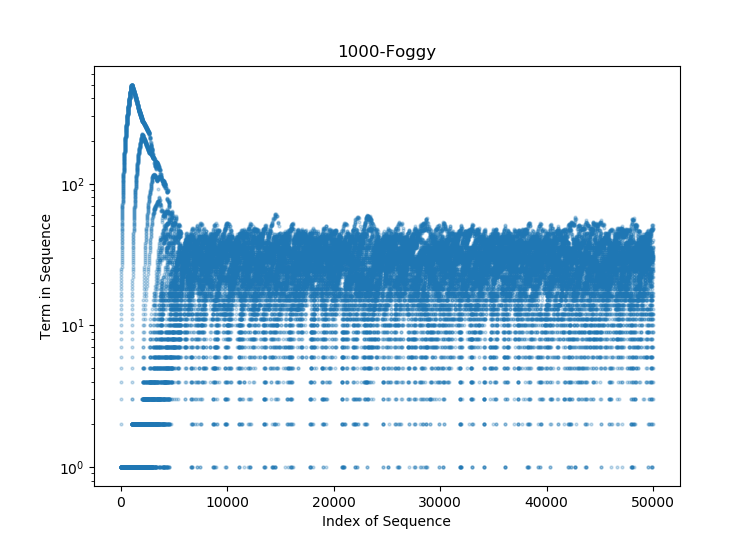
\includegraphics[scale=0.8]{figures/foggyExample.png}
 \caption{Here I would say something pithy and smart. \label{fig:foggyExample}}
\end{figure}

% TODO - add page number for Audioacive Decay article
\bibliographystyle{unsrt}  
\bibliography{references}  %%% Remove comment to use the external .bib file (using bibtex).
%%% and comment out the ``thebibliography'' section.


\end{document}